%\documentclass[10pt,dvipsnames,svgnames]{beamer}
\documentclass[aspectratio=169, lualatex, 10pt,dvipsnames,svgnames]{beamer} %
\makeatletter\def\input@path{{theme/}}\makeatother\usetheme{cipher}

\title{Computer Security: Introduction}
\author{Markulf Kohlweiss}
\subject{Introduction to Applied Cryptography covering cryptographic primitives, protocols, security goals, and real-world applications from basic concepts to advanced topics like TLS and zero-knowledge proofs.}
\keywords{cryptography, security, encryption, authentication, hash functions, TLS, protocols, provable security}
\institute{University of Edinburgh, School of Informatics}
\instituteimage{images/edu-white.png}
\date{\today}
\coversubtitle{INFR10067\\Fall 2025}
\coverpartname{Cryptography}
\covertopicname{Asymmetric encryption}
\coverwebsite{}


%\mode<presentation>
%{
%  \usetheme{default}
%  \usecolortheme{default}
%  \usefonttheme{default}
%  \setbeamertemplate{navigation symbols}{}
%  \setbeamertemplate{caption}[empty]
%  \setbeamertemplate{footline}[frame number]
%}

\iffalse
\setbeamertemplate{blocks}[rounded][shadow=true]
\setbeamercolor{block title}{fg=black, bg=Grey!50}
\setbeamercolor{block body}{fg=black, bg=Grey!25}
\setbeamercolor{block title alerted}{fg=black, bg=Red!20}
\setbeamercolor{block body alerted}{fg=black, bg=Red!15}
\setbeamercolor{block title example}{fg=black, bg=SeaGreen!20}
\setbeamercolor{block body example}{fg=black, bg=Green!15}
\fi

\usepackage[english]{babel}
\usepackage[utf8x]{inputenc}

\usepackage[lambda,advantage,operators,sets,adversary,landau,probability,notions,logic,ff,mm,primitives,events,complexity,asymptotics,keys]{cryptocode}

\usepackage{graphicx}
\usepackage{tikz}
\usetikzlibrary{arrows.meta}
\usetikzlibrary{shapes.geometric}
\pgfdeclarelayer{background}
\pgfsetlayers{background,main}

\usepackage{scrextend} 

\usepackage{fancybox}

\usepackage{pgfpages}

\usepackage{caption}
\usepackage{subcaption}

\usepackage{mdframed}
\usepackage{xspace}
\newcommand\Fontvi{\fontsize{5}{5.2}\selectfont}
\definecolor{ao}{rgb}{0.0, 0.6, 0.0}

\newcommand{\Inred}[1]{\textcolor{BrickRed}{#1}}
\newcommand{\Inblue}[1]{\textcolor{Blue}{#1}}
\newcommand{\Ingreen}[1]{\textcolor{SeaGreen}{#1}}

\newcommand{\V}[1]{\texttt{V\textsubscript{{#1}}}\xspace}
\newcommand{\Vs}[1]{$\texttt{V}'_\texttt{{#1}}$\xspace}
\newcommand{\BB}{\texttt{BB}\xspace}
\newcommand{\EA}{\texttt{EA}\xspace}
\newcommand{\A}{\adv\xspace}
\newcommand{\F}[1]{$\mathcal{F}_\textsc{{#1}}$\xspace}
\renewcommand{\S}{\sdv\xspace}
\newcommand{\E}{$\mathcal{E}$\xspace}
\renewcommand{\P}{$P$\xspace}
\newcommand{\D}{\ddv\xspace}

\newcommand{\Pt}[2]{$\Pi^{{#2}}_{\textsc{{#1}}}$\xspace}

\newcommand{\Enc}{\texttt{Enc}}
\newcommand{\CheckShares}{\texttt{Check}}

\newcommand{\ASetup}{\texttt{ASetup}}
\newcommand{\AEval}{\texttt{AEval}}
\newcommand{\AWit}{\texttt{AWit}}
\newcommand{\AVer}{\texttt{AVer}}

\newcommand{\CSetup}{\texttt{CSetup}}
\newcommand{\CCommit}{\texttt{CCommit}}
\newcommand{\COpen}{\texttt{COpen}}

\newcommand{\SGen}{\texttt{SGen}}
\newcommand{\SSign}{\texttt{SSign}}
\newcommand{\SVer}{\texttt{SVer}}

\newcommand{\SoKSetup}{\texttt{SoKSetup}}
\newcommand{\SoKSign}{\texttt{SoKSign}}
\newcommand{\SoKVer}{\texttt{SoKVer}}

\newcommand{\TLEnc}{\texttt{TLEnc}}
\newcommand{\TLDec}{\texttt{TLDec}}

\newcommand{\frameindent}{\hspace*{\baselineskip}}

\colorlet{gris}{black!50!white}
\def\engris#1{\textcolor{gris}{#1}}

\colorlet{jaune}{yellow!90!black}
\def\enjaune#1{\textcolor{jaune!70!black}{#1}}

\colorlet{vert}{green!45!black}
\def\envert#1{\textcolor{vert}{#1}}

\colorlet{bleu}{blue!70!black}
\def\enbleu#1{\textcolor{bleu}{#1}}

\colorlet{rouge}{red!75!black}
\def\enrouge#1{\textcolor{rouge}{#1}}

\newcommand{\rouge}{\only{\color{rouge}}}

\xdefinecolor{violet}{rgb}{.5,0,.7}
\def\enviolet#1{\textcolor{violet}{#1}}

\xdefinecolor{violetft}{rgb}{0.199,0., 0.398}
\def\envioletft#1{\textcolor{violetft}{#1}}

\xdefinecolor{monbleu}{rgb}{0,.2,.54}
\newcommand{\monbleu}{\only{\color{monbleu}}}

\newcommand{\Ccal}{\mathcal{C}}
\newcommand{\Kcal}{\mathcal{K}}
\newcommand{\Mcal}{\mathcal{M}}
\newcommand{\Tcal}{\mathcal{T}}
\newcommand{\Xcal}{\mathcal{X}}


\title{Cryptography: asymmetric encryption}

\author{Markulf Kohlweiss \\
  School of Informatics \\
  University of Edinburgh}



\date{}

\begin{document}

% \begin{frame}
% %\begin{center}
%    \includegraphics[scale=0.9]{images/silverplatter.pdf}\\
% %   \end{center}
%    How to do a PhD?\\
%    \pause
%    How to give a good lecture?\\
%    \pause
%    How to get the most out of your studies?

% \end{frame}

% \begin{frame}{Insecurity of MAC then Encrypt, Padding Oracle Attacks}

% \includegraphics[scale=0.4]{images/PaddingOracle.pdf}

% \engris{\url{https://crypto.stackexchange.com/questions/70570/how-does-the-cbc-padding-oracle-attack-work-in-general}}

% \end{frame}

\begin{frame}
  \maketitle
\end{frame}


\begin{frame}{Introduction}
  \vspace{-0.3cm}

  So far: how two users can protect data using a shared secret key
  \begin{itemize}
  \item One shared secret key per pair of users that want to communicate
    \begin{center}
      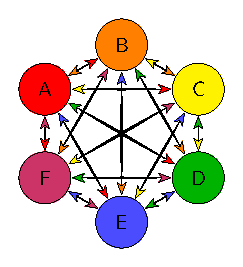
\includegraphics[scale=0.9]{images/SKD.pdf}
    \end{center}
  \end{itemize}

  Our goal now: how to establish a shared secret key to begin with?
  \begin{itemize}
  \item Trusted Third Party (TTP)
  \item Diffie-Hellman (DH) protocol
  \item $RSA$
  \item ElGamal (EG)
  \end{itemize}

\end{frame}

\begin{frame}{Recap}

  Action items:
  \begin{itemize}
  \item[$\checkmark$] Upload slides in advance (note that they might change before, and even after the lecture)\pause
  \item[$\checkmark$] Exercises: Those that struggle. please read this short chapter and do the exercises there: \url{https://joyofcryptography.com/pdf/chap0.pdf}\pause
  \item[$\checkmark$] \textbf{Office hours} are 11:15 Mon and Fri. 
  Talk with me after lecture, especially MSc students. \\ 
  Offer to discuss Feistel networks, S-boxes, and key schedules stands.\pause
  \item[$\checkmark$] Request: What are challenges in modern cryptography? \\ 
  Trusted, distributed, fair and safe AI. \textbf{Digital and Decentralized Identity.} Post-quantum. \\ Formalization of cryptography in theorem provers, e.g. Lean.
  \end{itemize}\medskip

  We finished MAC algorithms and authenticated encryption last time.

\end{frame}

\begin{frame}
\frametitle{Online Trusted Third Party (TTP)}

\begin{columns}[c]
\hspace{-1.0cm}
\begin{column}{0.40\textwidth}
      
  \begin{itemize}
  \item Users $U_1$, $U_2$, $U_3$, \dots, $U_n$, \dots
  \item Each user $U_i$ has a shared secret key $K_i$ with the TTP
  \item $U_i$ and $U_j$ can establish a key $K_{i,j}$ with the help of the TTP
  \item $\{m\}_k$ denotes the symmetric encryption of $m$ under the key $k$ \\ \ \\ \
   \end{itemize}
    \phantom{\enrouge{Question: can we establish a shared secret key without a TTP?}}
  \phantom{\enrouge{Answer: Yes!}}
\end{column}

\hspace{-0.8cm}
\begin{column}{0.55\textwidth}
  \begin{center}
    \includegraphics[scale=0.225]{images/Yahalom1.pdf}
    \captionof{figure}{Paulson's variant of the Yahalom protocol}
  \end{center}
\end{column}
\end{columns}
\end{frame}

\begin{frame}
\frametitle{Online Trusted Third Party (TTP)}

\begin{columns}[c]
\hspace{-1.0cm}
\begin{column}{0.40\textwidth}
      
  \begin{itemize}
  \item Users $U_1$, $U_2$, $U_3$, \dots, $U_n$, \dots
  \item Each user $U_i$ has a shared secret key $K_i$ with the TTP
  \item $U_i$ and $U_j$ can establish a key $K_{i,j}$ with the help of the TTP
  \item $\{m\}_k$ denotes the symmetric encryption of $m$ under the key $k$ \\ \ \\ \
   \end{itemize}
    \phantom{\enrouge{Question: can we establish a shared secret key without a TTP?}}
  \phantom{\enrouge{Answer: Yes!}}
\end{column}

\hspace{-0.8cm}
\begin{column}{0.55\textwidth}
  \begin{center}
    \includegraphics[scale=0.225]{images/Yahalom2.pdf}
    \captionof{figure}{Paulson's variant of the Yahalom protocol}
  \end{center}
\end{column}
\end{columns}
\end{frame}

\begin{frame}
\frametitle{Online Trusted Third Party (TTP)}

\begin{columns}[c]
\hspace{-1.0cm}
\begin{column}{0.40\textwidth}
      
  \begin{itemize}
  \item Users $U_1$, $U_2$, $U_3$, \dots, $U_n$, \dots
  \item Each user $U_i$ has a shared secret key $K_i$ with the TTP
  \item $U_i$ and $U_j$ can establish a key $K_{i,j}$ with the help of the TTP
  \item $\{m\}_k$ denotes the symmetric encryption of $m$ under the key $k$ \\ \ \\ \
   \end{itemize}
    \phantom{\enrouge{Question: can we establish a shared secret key without a TTP?}}
  \phantom{\enrouge{Answer: Yes!}}
\end{column}

\hspace{-0.8cm}
\begin{column}{0.55\textwidth}
  \begin{center}
    \includegraphics[scale=0.225]{images/Yahalom3.pdf}
    \captionof{figure}{Paulson's variant of the Yahalom protocol}
  \end{center}
\end{column}
\end{columns}
\end{frame}

\begin{frame}
\frametitle{Online Trusted Third Party (TTP)}

\begin{columns}[c]
\hspace{-1.0cm}
\begin{column}{0.40\textwidth}
      
  \begin{itemize}
  \item Users $U_1$, $U_2$, $U_3$, \dots, $U_n$, \dots
  \item Each user $U_i$ has a shared secret key $K_i$ with the TTP
  \item $U_i$ and $U_j$ can establish a key $K_{i,j}$ with the help of the TTP
  \item $\{m\}_k$ denotes the symmetric encryption of $m$ under the key $k$ \\ \ \\ \
   \end{itemize}
    \phantom{\enrouge{Question: can we establish a shared secret key without a TTP?}}
  \phantom{\enrouge{Answer: Yes!}}
\end{column}

\hspace{-0.8cm}
\begin{column}{0.55\textwidth}
  \begin{center}
    \includegraphics[scale=0.225]{images/Yahalom4.pdf}
    \captionof{figure}{Paulson's variant of the Yahalom protocol}
  \end{center}
\end{column}
\end{columns}
\end{frame}

\begin{frame}
\frametitle{Online Trusted Third Party (TTP)}

\begin{columns}[c]
\hspace{-1.0cm}
\begin{column}{0.40\textwidth}
      
  \begin{itemize}
  \item Users $U_1$, $U_2$, $U_3$, \dots, $U_n$, \dots
  \item Each user $U_i$ has a shared secret key $K_i$ with the TTP
  \item $U_i$ and $U_j$ can establish a key $K_{i,j}$ with the help of the TTP
  \item $\{m\}_k$ denotes the symmetric encryption of $m$ under the key $k$ \\ \ \\ \
   \end{itemize}
    \phantom{\enrouge{Question: can we establish a shared secret key without a TTP?}}
  \phantom{\enrouge{Answer: Yes!}}
\end{column}

\hspace{-0.8cm}
\begin{column}{0.55\textwidth}
  \begin{center}
    \includegraphics[scale=0.225]{images/Yahalom5.pdf}
    \captionof{figure}{Paulson's variant of the Yahalom protocol}
  \end{center}
\end{column}
\end{columns}
\end{frame}

\begin{frame}
  \frametitle{Goal of public-key encryption}
  \bigskip{}
    \centering
  \begin{tabular}{c}
    \hspace{-0.6cm}\includegraphics[scale=0.3]{images/padlock1.pdf}
  \end{tabular}
\end{frame}

\begin{frame}
  \frametitle{Goal of public-key encryption}
  \bigskip{}
  \centering
  \begin{tabular}{c}
    \hspace{-0.6cm}\includegraphics[scale=0.3]{images/padlock2.pdf}
  \end{tabular}
\end{frame}

\begin{frame}
  \frametitle{Goal of public-key encryption}
  \bigskip{}
    \centering
  \begin{tabular}{c}
    \hspace{-0.6cm}\includegraphics[scale=0.3]{images/padlock3.pdf}
  \end{tabular}
\end{frame}

\begin{frame}
  \frametitle{Goal of public-key encryption}
  \bigskip{}
    \centering
  \begin{tabular}{c}
    \hspace{-0.6cm}\includegraphics[scale=0.3]{images/padlock4.pdf}
  \end{tabular}
\end{frame}

\begin{frame}
  \frametitle{Goal of public-key encryption}
  \bigskip{}
    \centering
  \begin{tabular}{c}
    \hspace{-0.6cm}\includegraphics[scale=0.3]{images/padlock5.pdf}
  \end{tabular}
\end{frame}

\begin{frame}
  \frametitle{Goal of public-key encryption}
  \bigskip{}
    \centering
  \begin{tabular}{c}
    \hspace{-0.6cm}\includegraphics[scale=0.3]{images/padlock6.pdf}
  \end{tabular}
\end{frame}

\begin{frame}
  \frametitle{Public-key encryption - Definition}

  \begin{itemize}
  \item key generation algorithm: $G:\ \rightarrow \mathcal{K}_{pk}\times \mathcal{K}_{sk}$ 
    
    encryption algorithm $E:\ \mathcal{K}_{pk} \times \mathcal{M} \rightarrow \mathcal{C}$ 
    
    decryption algorithm $D:\ \mathcal{K}_{sk} \times \mathcal{C} \rightarrow \mathcal{M}$ 
    
    st. $\forall (sk, pk)\in G$, and $\forall m\in\mathcal{M}$, $D(sk, E(pk, m))\ =\ m$ 
    
    \begin{center}
      \includegraphics[scale=0.2]{images/encryptB.pdf}
    \end{center}

    
  \item the decryption key $sk_{Bob}$ is secret (only known to Bob). The
    encryption key $pk_{Bob}$ is known to everyone. And $sk_{Bob} \not= pk_{Bob}$

  \end{itemize}

\end{frame}

\coverpartname{Asymmetric encryption}
\covertopicname{We need a bit of number theory now}
\author{}
\date{}

\begin{frame}
  \maketitle
\end{frame}

\begin{frame}
  \frametitle{Primes}

  \begin{definition}
    $p\in\mathbb N$ is a {\bf prime} if its only divisors are 1 and $p$ 
  \end{definition}

  \envert{Ex: 2, 3, 5, 7, 11, 13, 17, 19, 23, 29}
  \bigskip{}
  \bigskip{}

  \begin{theorem}
    Every $n\in\mathbb N$ has a {\bf unique factorization} as a product of prime numbers (which are called its factors)
  \end{theorem}

  \envert{Ex: 23244 = 2 $\times$ 2 $\times$ 3 $\times$ 13 $\times$ 149}
\end{frame}

\begin{frame}
  \frametitle{Relative primes}

  \begin{definition}
    $a$ and $b$ in $\mathbb Z$ are {\bf relative primes} if they have no common factors
  \end{definition}
  \bigskip{}

  \begin{definition}
    The Euler function $\phi(n)$ is the number of elements that are relative primes with $n$:
    \[
    \phi(n) = |\{m \mid 0<m<n \text{ and } \mathsf{gcd}(m,n) = 1\}|
    \]
  \end{definition}
  \pause
  \begin{itemize}
  \item For $p$ prime: $\phi(p) =$ \pause $p\text{-}1$\pause
  \item For $p$ and $q$ primes: $\phi(p\cdot q) =$ \pause $(p\text{-}1)(q\text{-}1)$ 
  \end{itemize}
\end{frame}

\begin{frame}
  \frametitle{Integers modulo $n$: $\mathbb Z_n$}
  
  \begin{itemize}
  \item Let $n\in\mathbb N$. We define $\mathbb Z_n = \{0, \dots n\text{-}1\}$
    \[
    \forall a\in \mathbb Z_n,\ \forall b\in \mathbb Z,\ a \equiv b\ (\mathsf{mod}\ n)\ \Leftrightarrow\ \exists k\in\mathbb Z.\ b= a + k\cdot n
    \]
    \pause

  \item Modular inversion: the inverse of $x\in \mathbb Z_n$ is $y\in \mathbb Z_n$ \emph{s.t.} $x\cdot y \equiv 1\ (\mathsf{mod}\ n)$. We denote $x^{\text{-}1}$ the inverse of $x$ $\mathsf{mod}\ n$
    \pause

    \envert{Ex:\begin{tabular}[t]{l}
        $7^{\text{-}1}$ in $\mathbb Z_{12}$: \pause $7$\pause \\
        $4^{\text{-}1}$ in $\mathbb Z_{12}$: \pause \enrouge{$4$ has no inverse in $\mathbb Z_{12}$}
      \end{tabular}}
    \pause
  \begin{theorem}
    Let $n\in \mathbb N$. Let $x\in \mathbb Z_n$. $x$ has a inverse in $\mathbb Z_n$ iff $\mathsf{gcd}(x, n) = 1$
  \end{theorem}
  Inverse is computed using the Extended Euclidean Algorithm.
\end{itemize}
\end{frame}

\begin{frame}{Multiplicative group of integers modulo $n$: $\mathbb Z_n^*$}

  \begin{itemize}
  \item Let $n\in\mathbb N$. We define $\mathbb Z_n^* = \{x\in\mathbb Z_n\mid \mathsf{gcd}(x, n)=1\}$

    \envert{Ex: $\mathbb Z_{12} = \{1, 5, 7, 11\}$}
    \medskip{}
    \pause

  \item Note that $|\mathbb Z_n^*| = \phi(n)$
    \bigskip{}
    \pause

    \begin{theorem}[Euler]
      $\forall n\in\mathbb N$, $\forall x\in \mathbb Z_n^*$, $x^{\phi(n)} \equiv 1\ (\mathsf{mod}\ n)$
    \end{theorem}
    \bigskip{}
    \pause

    \begin{theorem}[Euler]
      $\forall p$ prime, $\mathbb Z_p^*$ is a cyclic group, \emph{i.e.}
      \[
      \exists g\in\mathbb Z_p^*,\ \{1, g, g^2, g^3, \dots, g^{p-2}\} = \mathbb Z_p^*
      \]
    \end{theorem}
  \end{itemize}
\end{frame}

\begin{frame}
  \frametitle{Intractable problems}
  \pause
\vspace{-0.3cm}
  
  \begin{itemize}
  \item \envert{\textsc{Factoring}:}

    \begin{tabular}[t]{l}
      input: $n\in\mathbb N$ \\
      output: $p_1,\dots, p_m$ primes \emph{st.} $n = p_1\cdot \dots \cdot p_m$
    \end{tabular}
    \medskip{}
    \pause

  \item \envert{\textsc{RSA Problem}}

    \begin{tabular}[t]{l}
      input:\begin{tabular}[t]{l}
        $n$ \emph{st.} $n=p\cdot q$ with $2\le p,q$ primes \\
        $e$ \emph{st.} $\mathsf{gcd}(e, \phi(n)) = 1$ \\
        $m^e\mod n$
      \end{tabular} \\
      output: $m$
    \end{tabular}
    \medskip{}
    \pause

  \item \envert{\textsc{Discrete Logarithm Problem (DLP)}:}

    \begin{tabular}[t]{l}
      input: prime $p$, generator $g$ of $\mathbb Z_p^*$, $y\in\mathbb Z_p^*$ \\
      output: $x$ such that $y = g^x\ (\mathsf{mod}\ p)$
    \end{tabular}
    \medskip{}
    \pause

  \item \envert{\textsc{Diffie-Hellman Problem (DHP)}:}

    \begin{tabular}[t]{l}
      input: prime $p$, generator $g$ of $\mathbb Z_p^*$, $g^a\ (\mathsf{mod}\ p)$, $g^b\ (\mathsf{mod}\ p)$ \\
      output: $g^{ab}\ (\mathsf{mod}\ p)$
    \end{tabular}
    \medskip{}

  \end{itemize}
\end{frame}

\coverpartname{Asymmetric encryption}
\covertopicname{Establish a key without a TTP}

\begin{frame}
  \maketitle
\end{frame}

\begin{frame}
  \frametitle{The Diffie-Hellman (DH) protocol}

  \begin{itemize}
  \item Assumption: the DHP is hard in $\mathbb Z_p^*$
  \item Fix a very large prime $p$, and $g$ generator of $\mathbb Z_p^*$
  \end{itemize}
  \pause

  \centering 
  \includegraphics[scale=0.3]{images/DH1.pdf}

\end{frame}

\begin{frame}
  \frametitle{The Diffie-Hellman (DH) protocol}

  \begin{itemize}
  \item Assumption: the DHP is hard in $\mathbb Z_p^*$
  \item Fix a very large prime $p$, and $g$ generator of $\mathbb Z_p^*$
  \end{itemize}

  \centering
  \includegraphics[scale=0.3]{images/DH2.pdf}

\end{frame}

\begin{frame}
  \frametitle{The Diffie-Hellman (DH) protocol}

  \begin{itemize}
  \item Assumption: the DHP is hard in $\mathbb Z_p^*$
  \item Fix a very large prime $p$, and $g$ generator of $\mathbb Z_p^*$
  \end{itemize}

  \centering
  \includegraphics[scale=0.3]{images/DH3.pdf}

\end{frame}

\begin{frame}
  \frametitle{The Diffie-Hellman (DH) protocol}

  \begin{itemize}
  \item Assumption: the DHP is hard in $\mathbb Z_p^*$
  \item Fix a very large prime $p$, and $g$ generator of $\mathbb Z_p^*$
  \end{itemize}

  \centering
  \includegraphics[scale=0.3]{images/DH4.pdf}

\end{frame}

\begin{frame}
  \frametitle{Man in the middle attack on DH}
  \centering
  \begin{tabular}{c}
    \hspace{-0.7cm}\includegraphics[scale=0.25]{images/DHattack1.pdf}
  \end{tabular}
\end{frame}

\begin{frame}
  \frametitle{Man in the middle attack on DH}
  \centering
  \begin{tabular}{c}
    \hspace{-0.7cm}\includegraphics[scale=0.25]{images/DHattack2.pdf}
  \end{tabular}
\end{frame}

\begin{frame}
  \frametitle{Man in the middle attack on DH}
  \centering
  \begin{tabular}{c}
    \hspace{-0.7cm}\includegraphics[scale=0.25]{images/DHattack3.pdf}
  \end{tabular}
\end{frame}

\begin{frame}
  \frametitle{Man in the middle attack on DH}
  \centering
  \begin{tabular}{c}
    \hspace{-0.7cm}\includegraphics[scale=0.25]{images/DHattack4.pdf}
  \end{tabular}
\end{frame}

\begin{frame}
  \frametitle{Man in the middle attack on DH}
  \centering
  \begin{tabular}{c}
    \hspace{-0.7cm}\includegraphics[scale=0.25]{images/DHattack5.pdf}
  \end{tabular}
\end{frame}

\begin{frame}
  \frametitle{Man in the middle attack on DH}
  \centering
  \begin{tabular}{c}
    \hspace{-0.7cm}\includegraphics[scale=0.26]{images/DHattack7.pdf}
  \end{tabular}
\end{frame}

\begin{frame}
  \frametitle{$RSA$ trapdoor permutation}
  \vspace{-0.4cm}

  \begin{itemize}
  \item $G_{RSA}() = (pk, sk)$ \hfill where $pk=(N, e)$ and $sk=(N,d)$

    \hfill and $N = p\cdot q$ with $p, q$ random primes

    \hfill and $e, d \in \mathbb Z$ st. $e\cdot d \equiv 1\ (\mathsf{mod}\ \phi(N))$
    \smallskip{}
    \pause

  \item $\Mcal = \Ccal = \mathbb Z_N$
   \smallskip{}
    \pause

  \item $RSA(pk, x) = x^e\ (\mathsf{mod}\ N)$ \hfill where $pk=(N,e)$
    \smallskip{}
    \pause

  \item $RSA^{\text{-}1}(sk, y) = y^d\ (\mathsf{mod}\ N) \hspace{2.25cm}$ \hfill where $sk=(N,d)$ 
    \smallskip{}
    \pause

  \item Correctness: $\forall (pk, sk) = G_{RSA}()$, $\forall x$, $RSA^{\text{-1}}(sk, RSA(pk, x)) = x$\medskip
    \pause

    \hspace{-1.0cm}\underline{Proof:} Let $pk = (N, e)$, $sk = (N, d)$. and $x\in\mathbb Z_N$. Easy case where $x$ and $N$ are relatively prime \pause
    \[
    \begin{array}[t]{lcl}
      RSA^{\text{-1}}(sk, RSA(pk, x)) & = & (x^e)^d\ (\mathsf{mod}\ N) \\\pause
                                    & = & x^{e\cdot d}\ (\mathsf{mod}\ N) \\\pause
                                    & = & x^{1 + k\phi(N)}\ (\mathsf{mod}\ N) \\\pause
                                    & = & x\cdot x^{k\phi(N)}\ (\mathsf{mod}\ N) \\\pause
                                    & = & x\cdot (x^{\phi(N)})^k\ (\mathsf{mod}\ N) \\\pause
                                    & \stackrel{\text{Euler}}{=} & x\ (\mathsf{mod}\ N) \\
    \end{array}
    \]
  \end{itemize}
\end{frame}

\begin{frame}
  \frametitle{How {\bf NOT} to use $RSA$}

  $(G_{RSA}, RSA, RSA^{\text{-}1})$ is called raw RSA (or sometimes Textbook RSA).\bigskip 
  
  Do not use raw RSA directly as an asymmetric cipher!\bigskip

  \enrouge{$RSA$ is deterministic and malleable $\Rightarrow$ not secure against chosen plaintext attacks}

\end{frame}

\begin{frame}
  \frametitle{ISO standard: ISO/IEC 18033-2}

  \mbox{Goal: build a CPA secure asymmetric cipher using $(G_{RSA}, RSA, RSA^{\text{-}1})$}
  \bigskip{}

  Let $(E_s, D_s)$ be a symmetric encryption scheme over $(\Mcal, \Ccal, \Kcal)$

  Let $H:\ \mathbb{Z}_N^*\rightarrow \Kcal$
  \bigskip{}

  Build $(G_{RSA}, E_{RSA}, D_{RSA})$ as follows
  \begin{itemize}
  \item $G_{RSA}()$ as described above
  \item $E_{RSA}(pk, m)$:
    \begin{itemize}
    \item pick random $x\in \mathbb Z_N^*$
    \item $y\leftarrow RSA(pk, x) \hfill (= x^e \mod\ N)$
    \item $k\leftarrow H(x)$
    \item return $y || E_s(k, m)$
    \end{itemize}
  \item $D_{RSA}(sk, y||c) = D_s(H(RSA^{\text{-}1}(sk, y)), c)$
  \end{itemize}
\end{frame}

\begin{frame}
  \frametitle{PKCS1 v2.0: RSA-OAEP (old version)}
  \bigskip{}

  \mbox{Goal: build a CCA secure asymmetric cipher using $(G_{RSA}, RSA, RSA^{\text{-}1})$}

  \begin{center}
    %\includegraphics[scale=0.09]{images/OAEP.png}
    \includegraphics[scale=0.45]{images/OAEP.pdf}
  \end{center}

\end{frame}

\begin{frame}
  \frametitle{PKCS1 v2.0: RSA-OAEP (wiki version)}
  \bigskip{}

  \mbox{Goal: build a CCA secure asymmetric cipher using $(G_{RSA}, RSA, RSA^{\text{-}1})$}

  \begin{center}
    \includegraphics[scale=0.09]{images/OAEP.png}
    %\includegraphics[scale=0.45]{images/OAEP.pdf}

  \end{center}

\end{frame}

\begin{frame}
  \frametitle{ElGamal (EG)}
\vspace{-0.3cm}

  \begin{itemize}
  \item Fix prime $p$, and generator $g\in\mathbb Z_p^*$
   \medskip{}
   \pause

  \item $\Mcal = \{0, \dots, p\text{-}1\}$ and $\Ccal = \Mcal \times \Mcal$
    \medskip{}
    \pause

  \item $G_{EG}() = (pk, sk)$ \hfill where $pk=g^d\ (\mathsf{mod}\ p)$ and $sk=d$

    \hfill and $d \stackrel{r}{\leftarrow} \{1, \dots, p\text{-}2\}$
    \medskip{}
    \pause


  \item $E_{EG}(pk, m) = (g^r\ (\mathsf{mod}\ p),\ m\cdot(g^d)^r\ (\mathsf{mod}\ p))$ 

    \hfill where $pk=g^d\ (\mathsf{mod}\ p)$
    
    \hfill and $r\stackrel{r}{\leftarrow} \mathbb Z$
    \medskip{}
    \pause

  \item $D_{EG}(sk, c) = e^{\text{-}d}\cdot f\ (\mathsf{mod}\ p) \hspace{2.25cm}$ \hfill where $c=(e,f)$ 
    \bigskip{}
    \pause

  \item Correctness: $\forall (pk, sk) = G_{EG}()$, $\forall m$, $D_{EG}(sk, E_{EG}(pk, m)) = m$\medskip
    \pause

    \hspace{-1cm}\underline{Proof:} Let $pk = g^d\ (\mathsf{mod}\ p)$ and $sk = d$\pause
    \vspace{-0.3cm}
    \[
    \begin{array}[t]{lcl}
      D_{EG}(sk, E_{EG}(pk, m)) & = & (g^r)^{-d}\cdot m\cdot(g^d)^r\ (\mathsf{mod}\ p) \\ \pause
                              & = & m\cdot g^{-rd}\cdot g^{rd}\ (\mathsf{mod}\ p) \\ \pause  
                              & = & m\ (\mathsf{mod}\ p) \\
    \end{array}
    \]
  \end{itemize}
\end{frame}

\end{document}
